\documentclass[10pt,a4paper]{article}
\usepackage[utf8]{inputenc}
\usepackage{amsmath}
\usepackage{amsfonts}
\usepackage{amssymb}
\usepackage{graphicx}

\begin{document}
\title{Projet 4: pre-labo 1}
\date\today
\author{Groupe 7}
\maketitle

\section{Calcul de la différence de temps}
	Afin d'observer les répliques, une configuration a été pensée (Figure \ref{conf1} et \ref{conf2}). $d$ est la distance $Tx$ et $Rx$ alors que $x$ est la distance minimale entre $Rx$ (ou $Tx$) et la plaque. Le temps que met l'onde pour passer de $Rx$ à $Tx$ est donné par l'équation \ref{t1}. L'équation \ref{t2} donne le temps du trajet de l'onde réfléchie sur la plaque. $c$ est la vitesse de la lumière. 	

	\begin{equation}
	t_1 = \frac{d}{c}
	\label{t1}
	\end{equation}
	
	\begin{equation}
	t_2 = \sqrt{(\frac{d}{2})^2 + x^2} * \frac{1}{c}
	\label{t2}
	\end{equation}
	
	Le première situation sera réalisée pour obtenir un grand $\Delta t$ alors que la seconde pour en obtenir un plus grand.
	\begin{equation}
	\Delta t = t_2 - t_1 = (\sqrt{(\frac{d}{2})^2 + x^2} - d ) * \frac{1}{c}
	\end{equation}
	
	\begin{figure}[h]
	\centering
	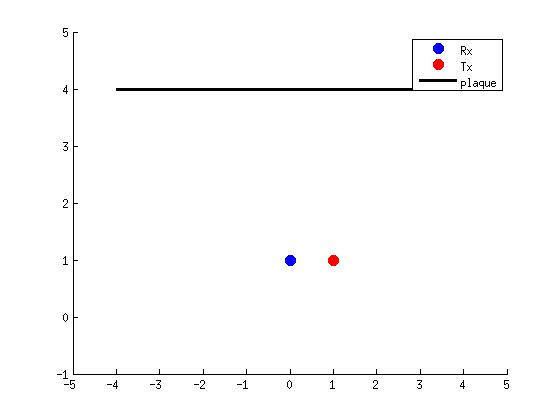
\includegraphics[scale=0.4]{conf1.jpg}
	\caption{Première configuration \label{conf1} }
	\end{figure}		
	
	\begin{figure}[h]
	\centering
	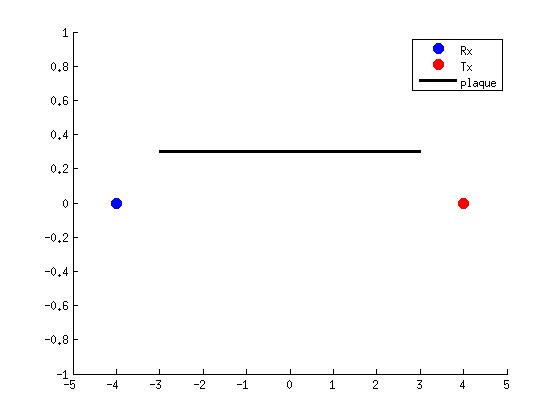
\includegraphics[scale=0.4]{conf2.jpg}
	\caption{Deuxième configuration \label{conf2}}
	\end{figure}		
	
	
	\section{Détermination des paramètres géométriques}
		Afin de ne pas avoir de recouvrement entre deux répliques d'une impulsion, il faut que $\Delta t$ soit plus grand que le temps d'une impulsion ($2.5ps$).
		
		
		\begin{figure}[h]
		\centering
		\begin{tabular}{|l|l|l|l|}
		\hline
		 configuration & $\Delta t [ns]$ & $d [m]$ & $x [m]$ \\
		 \hline
		 1 & $3$ & $2$ & $1.0496$ \\
		 2 & $4$ & $2$ & $1.2485$ \\
		 3 & $6$ & $1$ & $1.3070$ \\
		 4 & $8$ & $0.3$ & $1.3408$ \\
		 5 & $10$ & $0.3$ & $1.6421$ \\
		 \hline
		\end{tabular}
		
		\caption{Set-up pour le premier labo}
		\end{figure}

\end{document}
